\documentclass[12pt]{article}
\usepackage{fullpage}
\usepackage{amssymb, amsthm, amsmath}
%\usepackage{doublespace}
\usepackage{bm}
\usepackage{graphicx}
\usepackage{subfig}
\usepackage[authoryear]{natbib}
\usepackage{bm}
\usepackage{verbatim}
\usepackage{lineno}
\usepackage{times}
\usepackage{caption}
%\usepackage{subcaption}
\usepackage{epstopdf}
\usepackage{multicol}
\usepackage{afterpage}

\linespread{1}

\newcommand{\btheta}{ \mbox{\boldmath $\theta$}}
\newcommand{\bmu}{ \mbox{\boldmath $\mu$}}
\newcommand{\balpha}{ \mbox{\boldmath $\alpha$}}
\newcommand{\bbeta}{ \mbox{\boldmath $\beta$}}
\newcommand{\tbeta}{ \mbox{$\tilde \beta$}}
\newcommand{\bdelta}{ \mbox{\boldmath $\delta$}}
\newcommand{\blambda}{ \mbox{\boldmath $\lambda$}}
\newcommand{\bgamma}{ \mbox{\boldmath $\gamma$}}
\newcommand{\brho}{ \mbox{\boldmath $\rho$}}
\newcommand{\bpsi}{ \mbox{\boldmath $\psi$}}
\newcommand{\bepsilon}{ \mbox{\boldmath $\epsilon$}}
\newcommand{\bomega}{ \mbox{\boldmath $\omega$}}
\newcommand{\bDelta}{ \mbox{\boldmath $\Delta$}}
\newcommand{\bSigma}{ \mbox{\boldmath $\Sigma$}}
\newcommand{\boldeta}{ \mbox{\boldmath $\eta$}}
\newcommand{\bone}{ \mbox{\boldmath $1$}}
\newcommand{\bA}{ \mbox{\bf A}}
\newcommand{\ba}{ \mbox{\bf a}}
\newcommand{\bP}{ \mbox{\bf P}}
\newcommand{\bx}{ \mbox{\bf x}}
\newcommand{\bX}{ \mbox{\bf X}}
\newcommand{\bB}{ \mbox{\bf B}}
\newcommand{\bZ}{ \mbox{\bf Z}}
\newcommand{\by}{ \mbox{\bf y}}
\newcommand{\bY}{ \mbox{\bf Y}}
\newcommand{\bz}{ \mbox{\bf z}}
\newcommand{\bh}{ \mbox{\bf h}}
\newcommand{\br}{ \mbox{\bf r}}
\newcommand{\bt}{ \mbox{\bf t}}
\newcommand{\bs}{ \mbox{\bf s}}
\newcommand{\bb}{ \mbox{\bf b}}
\newcommand{\bL}{ \mbox{\bf L}}
\newcommand{\bu}{ \mbox{\bf u}}
\newcommand{\bg}{ \mbox{\bf g}}
\newcommand{\bv}{ \mbox{\bf v}}
\newcommand{\bV}{ \mbox{\bf V}}
\newcommand{\bG}{ \mbox{\bf G}}
\newcommand{\bH}{ \mbox{\bf H}}
\newcommand{\bD}{ \mbox{\bf D}}
\newcommand{\bM}{ \mbox{\bf M}}
\newcommand{\bw}{ \mbox{\bf w}}
\newcommand{\bo}{ \mbox{\bf o}}
\newcommand{\bfe}{ \mbox{\bf e}}
\newcommand{\iid}{\stackrel{iid}{\sim}}
\newcommand{\indep}{\stackrel{indep}{\sim}}
\newcommand{\calR}{{\cal R}}
\newcommand{\calG}{{\cal G}}
\newcommand{\calD}{{\cal D}}
\newcommand{\calS}{{\cal S}}
\newcommand{\calB}{{\cal B}}
\newcommand{\calA}{{\cal A}}
\newcommand{\calT}{{\cal T}}
\newcommand{\calO}{{\cal O}}
\newcommand{\calGP}{{\cal GP}}
\newcommand{\mR}{{\cal R}}
\newcommand{\mC}{{\cal C}}
\newcommand{\argmax}{{\mathop{\rm arg\, max}}}
\newcommand{\argmin}{{\mathop{\rm arg\, min}}}
\newcommand{\Frechet}{\mbox{Fr$\acute{\mbox{e}}$chet}}
\newcommand{\Matern}{ \mbox{Mat$\acute{\mbox{e}}$rn}}
\newcommand{\PM}{ \mbox{PM$_{2.5}$}}

\def\sgn{\mathrm{sgn}}
\def\STGP{\mathcal{STGP}}


\newcommand{\beq}{ \begin{equation}}
\newcommand{\eeq}{ \end{equation}}
\newcommand{\beqn}{ \begin{eqnarray}}
\newcommand{\eeqn}{ \end{eqnarray}}
\newtheorem{corollary}{Corollary}
\newtheorem{proposition}{Proposition}
\newtheorem{lemma}{Lemma}
\newtheorem{theorem}{Theorem}

\newtheorem{mydef}{Definition}
\newtheorem{mythm}{Theorem}
\newtheorem{mylemma}{Lemma}
\newtheorem{myproposition}{Proposition}
\newtheorem{mycor}{Corollary}


\begin{document}\linenumbers

\graphicspath{ {Figures/} }

\begin{center}
{\Large {\bf Lymphoblastoid Cell Lines as a Model System for Chemotherapy Response in Breast Cancer Patients - Exploratory Analysis Report}}\\
\large{Jeremy Ash, Alexandra Larsen} \\
\today
\end{center}

\section*{Summary of Data Analysis}\label{s:intro}

\begin{enumerate}
	\item Visualization: basic statistical graphics, correlations and PCA
	\item Significance Testing:  MANOVA, simple and multiple linear regression
	\item Model Fitting
	\item Variable Selection
\end{enumerate}

\section*{Introduction}

Lymphoblastoid cell lines (LCLs) are a commonly used model system for pharmacogenomic studies. Previous research has shown these immortalized cells to be good surrogates for lymphocytes, suggesting that LCLs may be an appropriate model for in-vivo drug exposure. LCLs are a promising candidate for a model system as they present relatively few confounding variables compared to clinical trials, the common approach to studying in-vivo drug exposure. Additionally, using an LCL model system allows for avoiding complications that arise within clinical trials, such as changes in treatment regimen and experimental design problems. However, there still may be limitations to translating in-vitro LCL drug exposure to in-vivo outcomes.  For example, LCLs are often not from tissue where drug response is of interest, which makes them questionable as a model system. This motivates extensive research into LCLs as effective model systems. Using a novel data set that includes both in-vivo and in-vitro data from breast cancer patients, we conduct an exploratory analysis of relationships between in-vitro dose response data and clinical outcomes designed to provide insight to Alison and collaborators on LCLs as a model system. 

\newpage

\section{Data}

We have in-vivo and in-vitro data from 93 clinical trial participants who received Taxane chemotherapy treatment for breast cancer. \\

The in-vivo data include variables on 
\begin{itemize}
	\item Treatment regimens (dosing interval, chemo regimen, total weeks of treatment, number of cycles)
	\item Pre-study cancer status (tumor grade, cancer stage)
	\item Additional patient data (age, race, smoking status, menopause status, Her2-positivity and estrogen receptor positivity)
	\item Post-study cancer status, recovery status, extent of recovery and toxicity reactions (myalgia, neuropathy, neutropenia, cancer stage)
\end{itemize}
\begin{figure}[h]
\caption{Example of the QC in-vitro dose-response data (left) and the composite dose-response curve fit to the data (right).  The figure on the right indicates the location of the AC50 value extracted from the composite curve. (Figure courtesy of John Jack)}
\centering
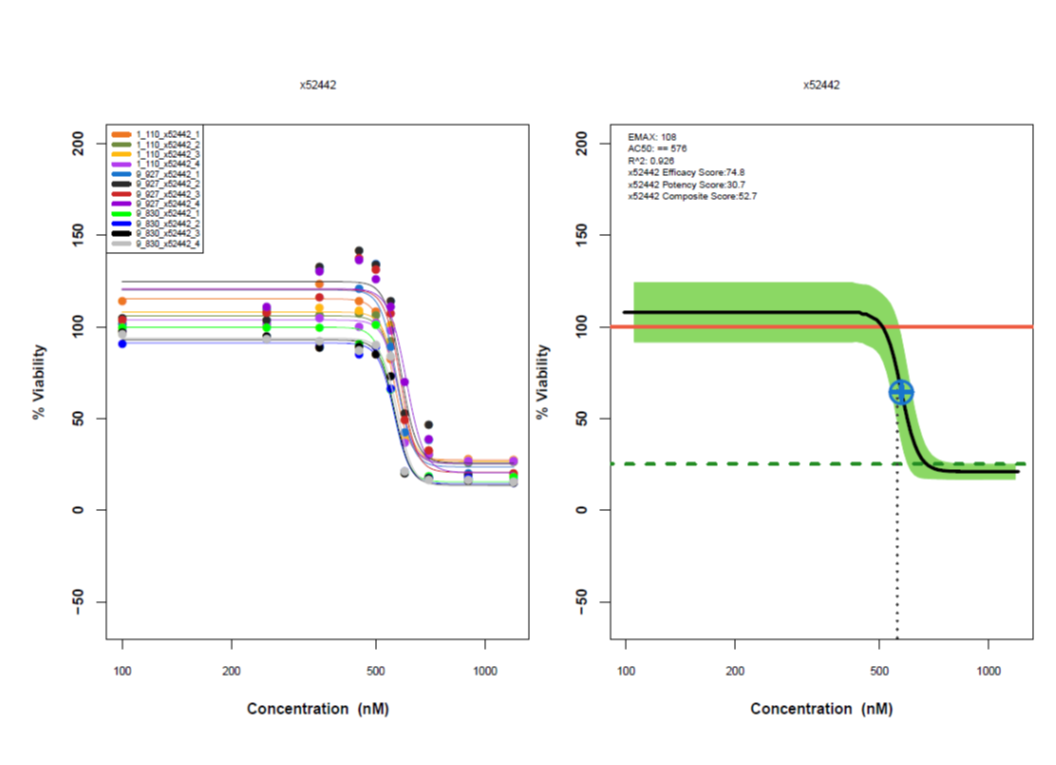
\includegraphics[width=0.85\textwidth]{CompositeCurve.png}
\end{figure}
We note that several of our measurements suffer from imbalanced classes and large outliers. Some of the patients in this study underwent surgery as part of their treatment and while not considered in this report, this information could be gleaned from the data for inclusion in further study. \\

A total of 93 Lymphoblastoid cell lines (LCL's) were cultured from each patient and immortalized with Epsten-Barr virus. Percent viability for each cell line was measured at each of 10 increasing dosages (nM) of Paclitaxel (100, 250, 350, 450, 500, 550, 600, 700, 900, 1200). Initially, each cell line had data for approximately 12 replicate dose-response experiments.  An extensive QC pipeline - designed by John Jack, Alison Motsinger-Reif and collaborators - was applied to this data.  We also used curves fit to the data by John Jack to compute the AC50 (the concentration at which there is 50\% viability).  We used this as a summary measure of the dose-response curves. Figure 1 displays the QC dose-response curve for one patient, as well as the composite curve fit to the data. \\

\afterpage{%
\begin{figure}[h]
\caption{Examples of QC pipeline data (Figures Courtesy of John Jack)}
\centering
\subfloat[Pre Monotonic Filter
]{
  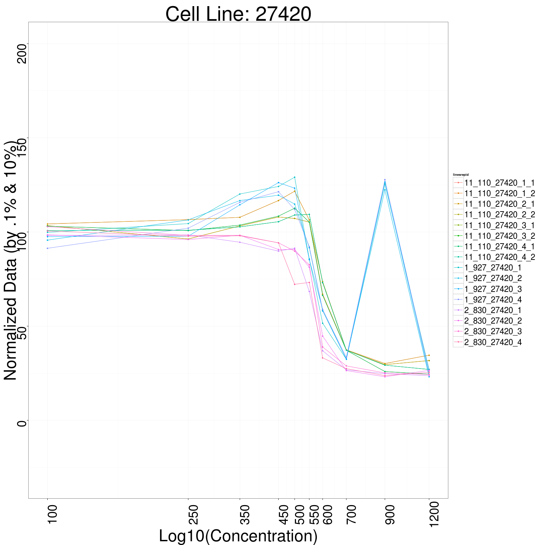
\includegraphics[width=0.45\textwidth]{QC2}
}
\subfloat[Post Monotonic Filter
]{
  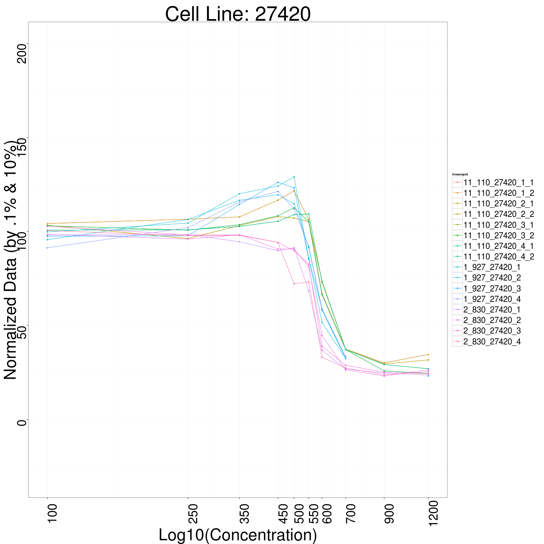
\includegraphics[width=0.45\textwidth]{QC3}
}
\hspace{0mm}
\subfloat[Typical Data Post QC]{
  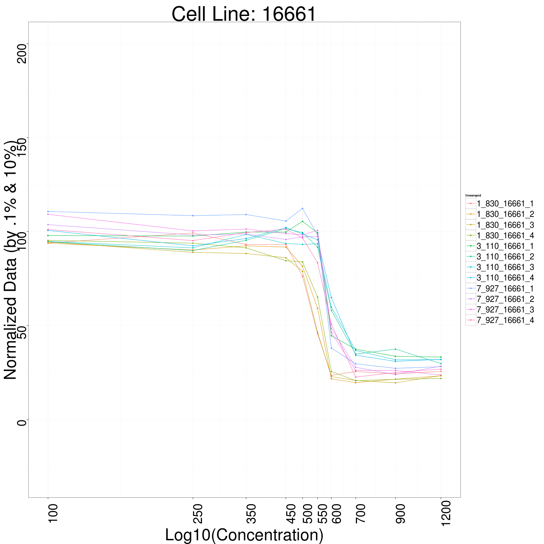
\includegraphics[width=0.45\textwidth]{QC1}
}
\subfloat[Remaining problematic data]{
  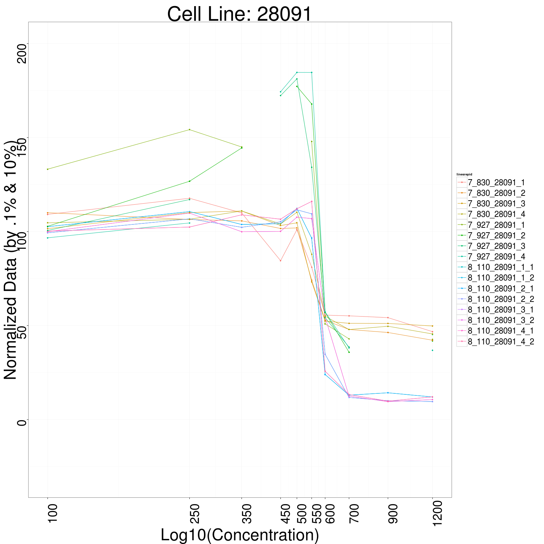
\includegraphics[width=0.45\textwidth]{QC4}
}
\end{figure}
\clearpage
}



A brief outline of the QC pipeline follows.
For step 1 of the QC pipeline, coefficient of variation smoothing of the data was performed.  In step 2, the plates were checked for an abnormally low 90th percentile of cell counts. No plates had a 90th percentile below 2500, and none were removed. For step 3, cell counts for each cell line were normalized to positive and negative controls such that the cell count for the negative control (.1\% DMSO) was considered 100\% viability and the cell count at the positive control (10\% DMSO) was considered 0\% viability.  For step 4, a monotonicity filter was performed.  If there was an increase in viability by 30\% or more as the concentration of Paciltaxel increased, the data was discarded. These points were very large outliers that would present difficulties in model fitting, and they were likely due to experimental error. Finally, the mean percent viabilities were computed using the remaining replicates for each patient.  Figure 2a and Figure 2b show that the monotonicity filter was necessary and is able to mostly remove the remaining large outliers. Figure 2c highlights the fact that the majority of dose-response data post QC pipeline is devoid of large outliers.  However, Figure 2d shows an example of an anomaly where the QC process could be improved.  Since some large outliers still remain in the data, and these will have a large influence on the means computed at the end of the QC pipeline, perhaps it would be prudent to redo our analysis using another measure like the median to summarize the dose-response replicates.\\

\section{Data Visualization}

To visually explore the relationship among in-vivo and in-vitro variables, we constructed basic statistical graphics, calculated correlations and ran PCA. All additional figures, data, and analyses not shown in this report will be made available to Alison in a folder containing all the files relevant to our analysis.  
\subsection{Single Variable Plots and Descriptions}


For continuous variables we used box plots, histograms and summary measures of the distributions to examine variation and distribution shape. Figure 3a shows that several of the dose-response variables have a few very large outliers.  These may need to examined further in subsequent analyses.  These outliers are likely due to the occasional large outliers in the dose-response data that were not smoothed during the QC process.  For categorical variables, we created bar plots and frequency tables.  Figure 3b demonstrates how many of the categorical variables are highly imbalanced.\\

We considered the ordinal variable, in-vivo response to Taxane, as both continuous and categorical, due to the fact that the variable was treated as both data types, depending on the analysis performed.
\begin{figure}[h]
\caption{Interesting single variable plots}
\centering
\subfloat[Large outliers]{
  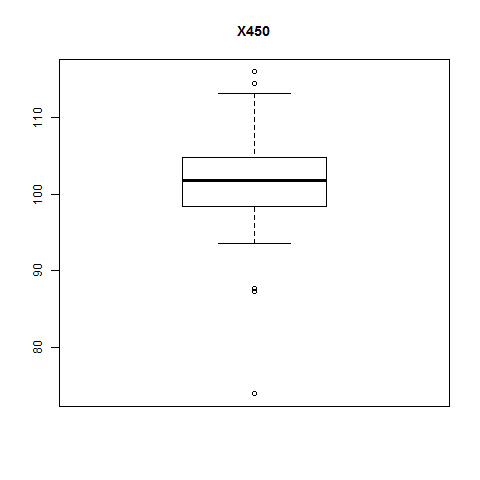
\includegraphics[width=65mm]{X450boxplot.png}
}
\subfloat[Imbalanced classes]{
	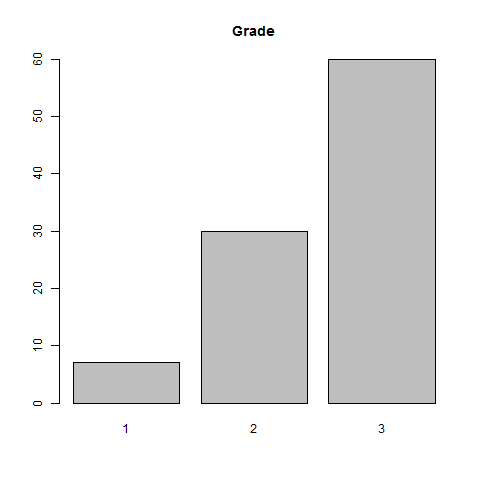
\includegraphics[width=65mm]{Gradebarplot.png}
}
\end{figure}
\begin{figure}[h]
\caption{Continous by continuous variable associations}
\centering
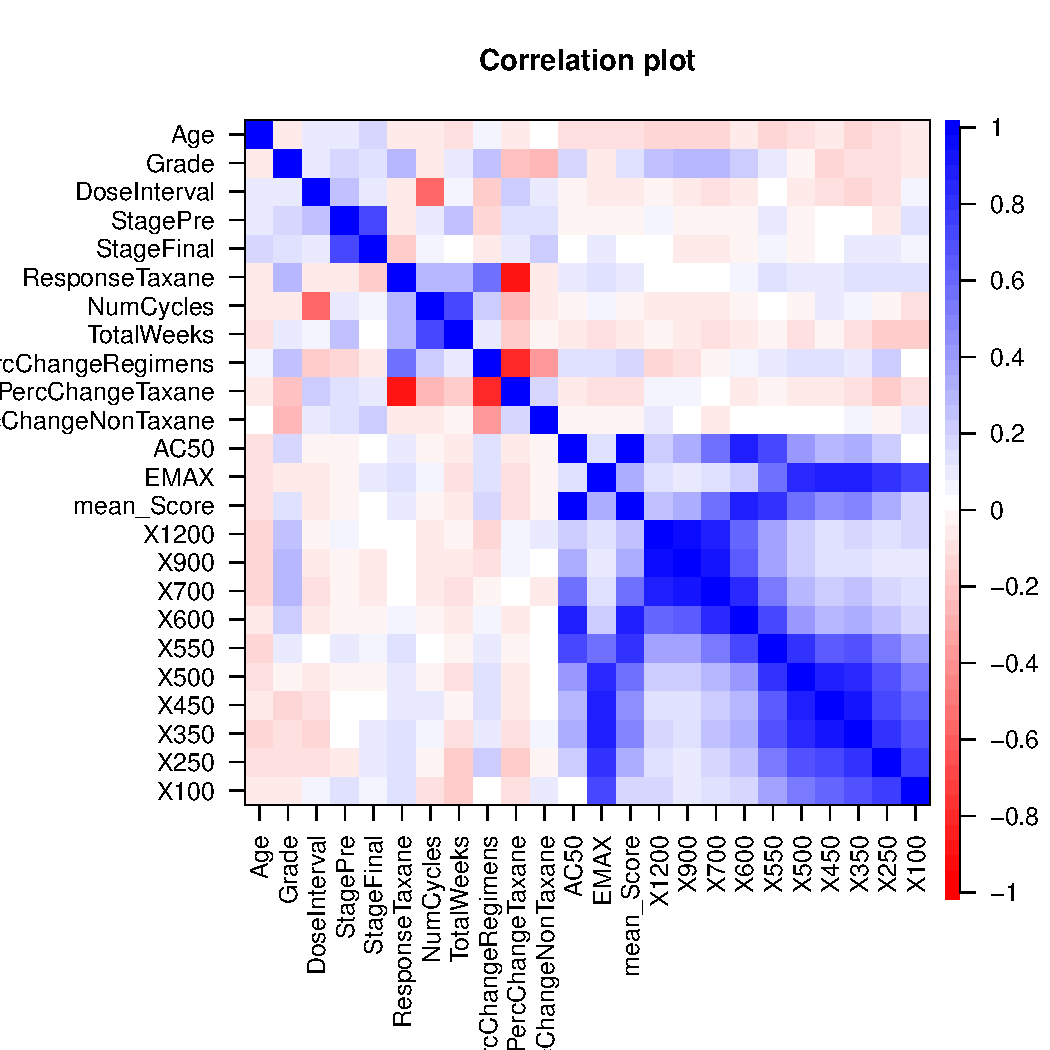
\includegraphics[width=0.85\textwidth]{contCor}
\end{figure}

\begin{figure}[h]
\caption{Categorical by categorical variable associations}
\centering
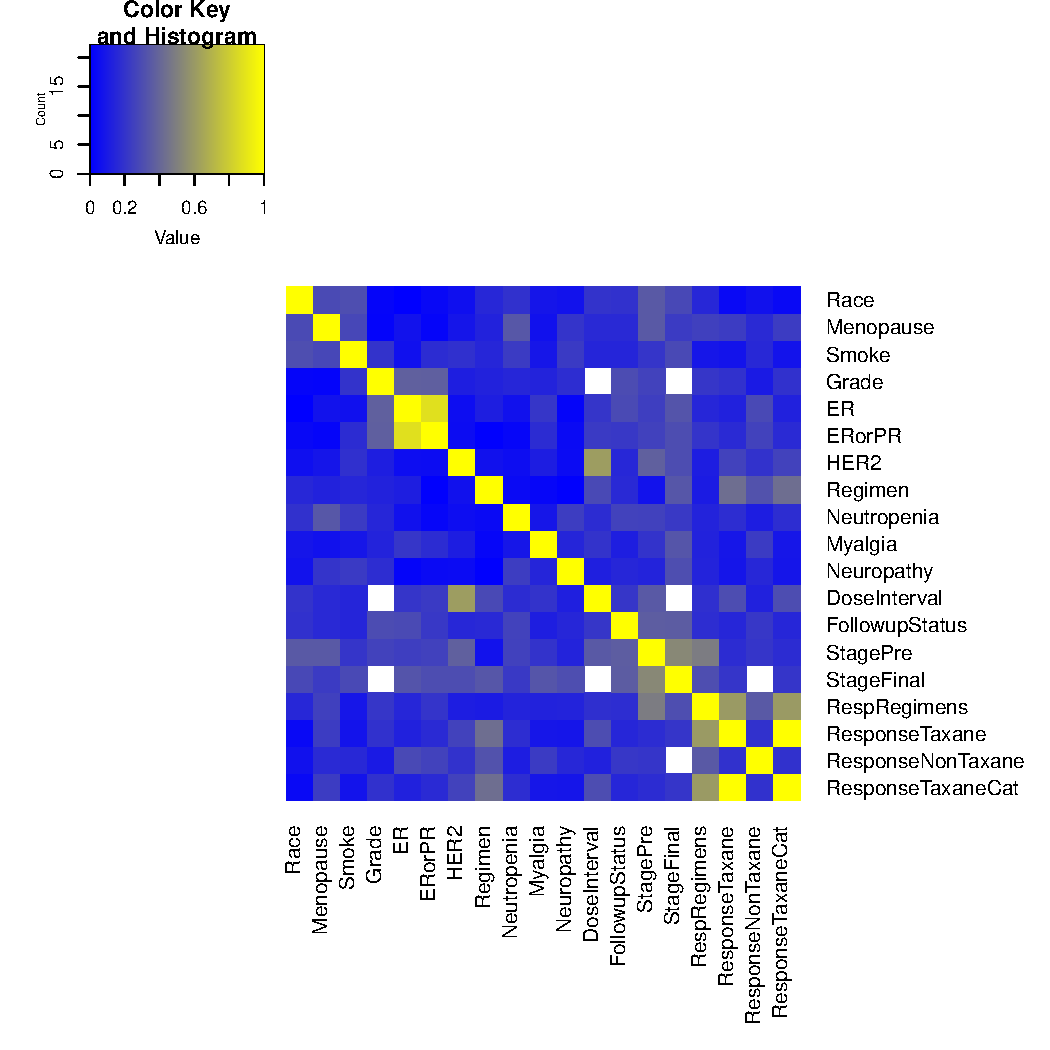
\includegraphics[width=0.85\textwidth]{CramerV}
\end{figure}

\begin{figure}[h]
\caption{Categorical by continuous variable associations}
\centering
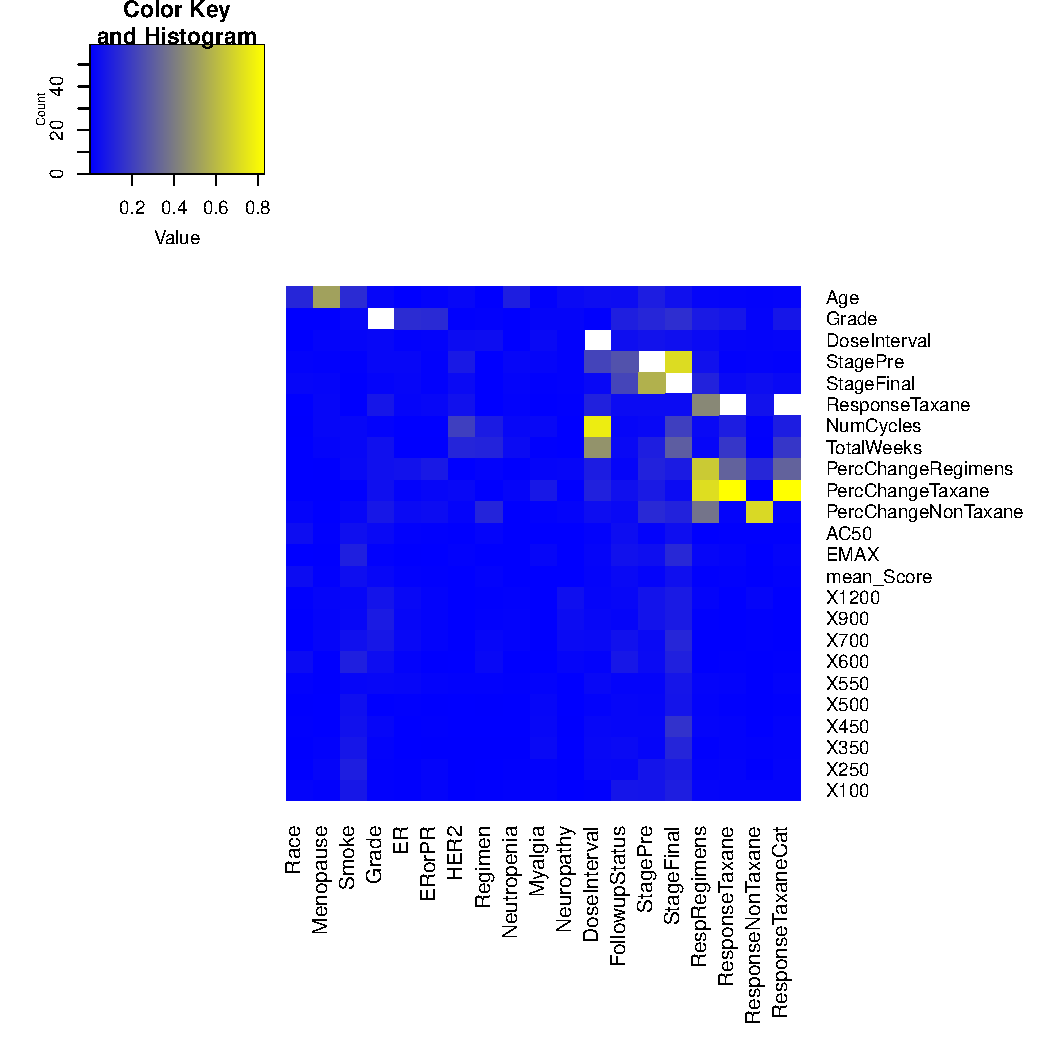
\includegraphics[width=0.85\textwidth]{etaSQ}
\end{figure}
\begin{figure}[h]
\caption{Dose-response variable scatterplots colored by in-vivo response to Taxane variable}
\centering
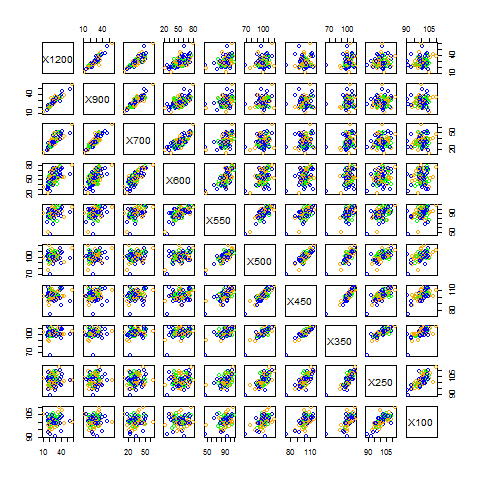
\includegraphics[width=0.85\textwidth]{pairPlot}
\end{figure}

\begin{figure}[h]
\caption{Principle components analysis}
\centering
\subfloat[Biplot with PCA scores and loadings]{
  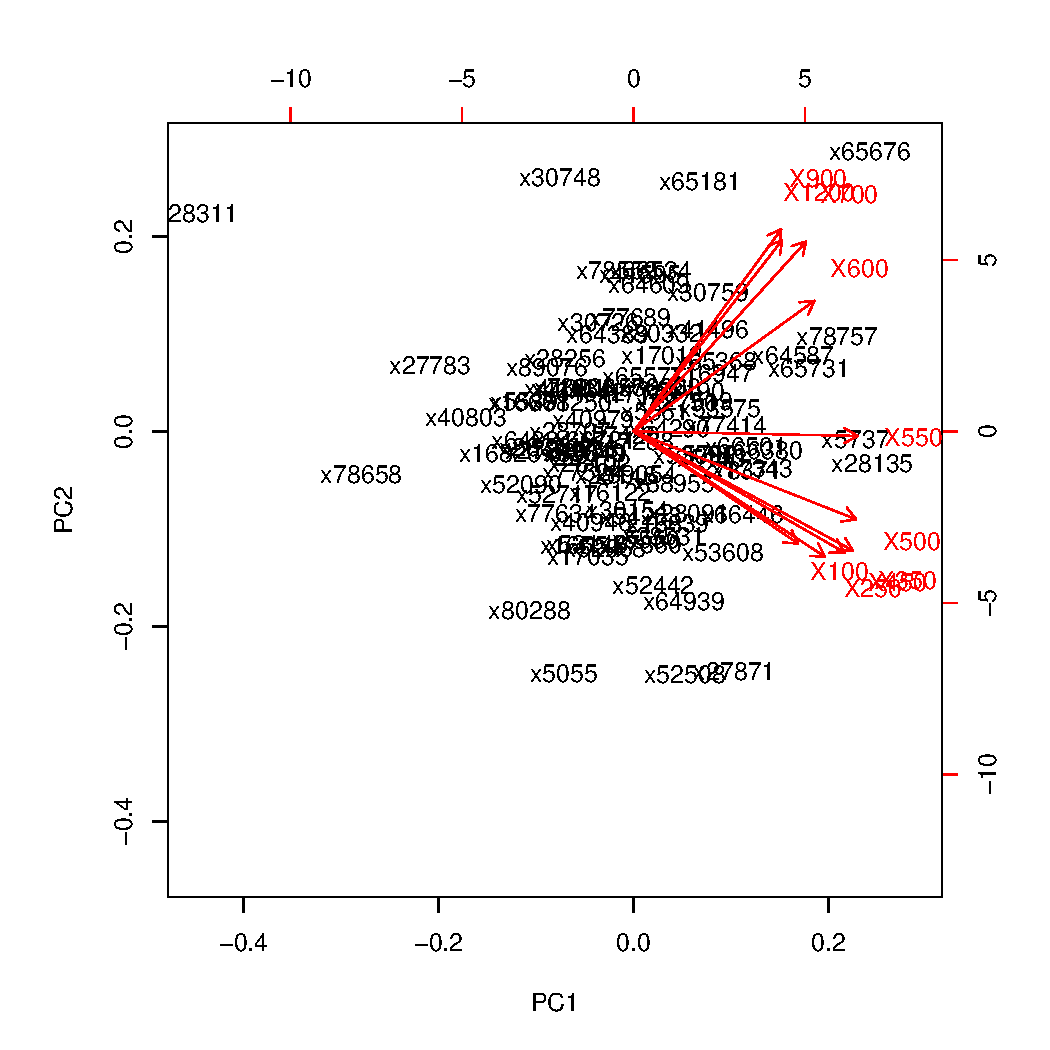
\includegraphics[width=0.45\textwidth]{pcaResponseClassLoadings}
}
\subfloat[PCA with points colored by response to Taxane]{
  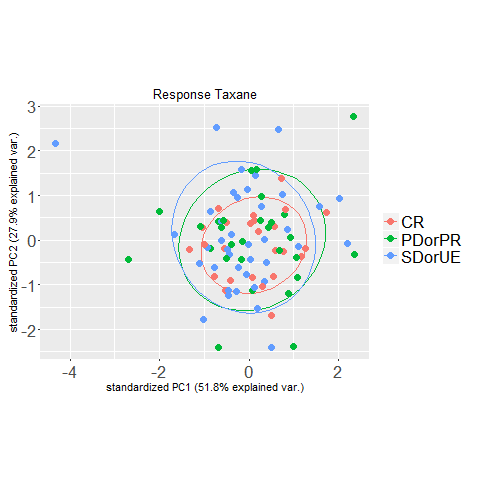
\includegraphics[width=0.45\textwidth]{pcaResponseClass}
}
\end{figure}
\subsection{Pairwise Associations}
We also analyzed all pairwise relationships between variables.  We computed Pearson correlations among continuous variables (Figure 4).  There are no continuous variables that are strongly associated with AC50, other than other in-vitro dose-response variables, which is trivial.  There also no continuous variables strongly associated with the ReponseTaxane variable, other than PercChangeRegimens and PerChangeTaxane, which are similar measures of clinical outcome. However, there are strong correlations between other variables, like the dose-response variables.  These variables will need to be considered carefully during model building. Cramer's V method was used to compute association among categorical variables (Figure 5).  Again, there are no variables associated with ResponseTaxane other than the aforementioned trivial variables. There are strong associations between other categorical variables, though.  To investigate these associations further, mosaic plots were constructed for all pairwise comparisons of categorical variables.  An example of the usefulness of these plots is demonstrated in Figure 11a, where we investigate the association between the Race and Smoke variables.  We also performed an ANOVA to compare the continuous and categorical variables and computed $\eta^2$ to measure the strength of associations (Figure 6). There are empty cells where ANOVA could not be performed.  There are no strong associations with AC50, and only strong associations between ResponseTaxane and trivial clinical outcome variables.  Interestingly, TotalWeeks and NumCycles are associated with StageFinal, and StageFinal shows a moderate association with the dose-response variables.\\

Figure 7 shows the scatterplot matrix for all of the in-vitro dose-response variables.  Each point represents a patient cell line and the colors indicate in-vivo response to Taxane. Green, orange, and blue represent complete recovery, partial recovery, and no recovery, respectively.   First, it is clear from these scatterplots that the dose-response variables are highly correlated.  However, these plots reinforce that there does not appear to be any linear association between the dose-response variables and the in-vivo response to Taxane variable.  Therefore, we do not expect that a linear model that uses the dose-response variables to predict in-vivo response to Taxane to perform well.  (Scatterplots between all variables can be found in the figures folder.)
\subsection{Principle Components Analysis}
However, it is still possible that there is strong multicollinearity between the in-vivo response to Taxane and the in-vitro dose-response variables.  To more generally investigate whether the dose-response variables could be used to predict either a categorical or quantitative version of in-vivo response to Taxane, a principle components analysis (PCA) was performed (Figure 6).  Each point in these plots represents a patient's dose-response profile (10 dose-response variables).  Since the plot of the first two principle components (PCs) is the best estimate of the position of the points in two dimensions, we can use this plot to estimate whether cell lines with similar dose-response curves have similar in-vivo response to Taxane.  79.7\% of the variation in the dose-response variables is explained in the first two principle components (PCs) due the fact that many of variables are highly correlated. Therefore, this plot is a very good representation of the dose-response data. Figure 8a is a biplot showing the principle components scores for each cell line along with the loadings. The high concentration response variables (X600 - X1200) have similar loadings, as do the low concentration response variables (X100 - X500). This is because the percent viabilities are fairly constant across these concentration ranges.  All of the X550 variable variation is along the first PC.  The X550 concentration is near the AC50 concentration for all dose-response curves.  Figure 8b colors the points by the in-vivo response to Taxane.  There is no clear difference between the dose-response curves of patients with different in-vivo responses to Taxane.  If we were to use a classification method, the decision boundary is likely very non linear.  These results suggest that a inflexible model like a linear model using the dose-response variables as predictors may have difficulty predicting in-vivo response to Taxane.  However, a flexible model like a tree based method which divides predictor space into distinct regions and then makes predictions using the average response in each regions may perform well.  PCA plots comparable to Figure 8b where points are colored by every other in-vivo variable can be found in the figures folder.

\iffalse
All figure captions should explain what information we're getting from the graphics: \\
\textbf{Figure 1}: Interesting box plots \\
\textbf{Figure 2}: Correlation matrices \\
\textbf{Figure 3}: Interesting PCA plots\\
\textbf{Figures}: [JEREMY:] What am I missing; do we want to include the tri-colored DRC (dose-response curve) pairs plot?
\fi

\section{Significance Testing}
\subsection{Clinical data and full dose-response curve}

We performed one way MANOVA analyses using the dose-response variables as the response and each in-vivo variable of interest as grouping variables.  Our results indicate that race and smoking status are  significant after correcting for multiple comparisons (Table 1).  To control the False Discovery Rate (FDR; proportion of false positives) we compare raw p-values to the Benjamini-Hochberg critical value (BHCV) and set the FDR to 10\%. Histograms of the dose-response variables can be found in the figures folder, along with summary statistics of their distributions.  We were concerned about normality due to our small sample size.  Each distribution is approximately normal, but a more thorough check of the multivariate normality of residuals may need to be performed.  Figure 9 highlights some of the challenges the data presented during MANOVA analysis. Figure 9a shows the extremely high correlation between the dose-response variables.  Highly correlated response variables (above .7 Pearson's correlation) are known to decrease the power of MANOVA (see \textit{Iacobucci, Dawn (ed.) (2001), Journal of Consumer Psychology's Special Issue on Methodological and Statistical Concerns of the Experimental Behavioral Researcher, 10 (1\&2), Mahwah, NJ: Lawrence Erlbaum Associates, 5-35.}).  To address this problem we took one dose-response variable from each highly correlated block. Four dose-response variables remained after this step (X1200, X600, X500, and X100).  We took the highest and lowest concentration variables to maintain the full range of the dose-response curves.  When the MANOVA analysis was run without this filtering step, no significant associations were found after correcting for multiple testing.  \\

Figure 9b shows the highly imbalanced class problem again.  Since the power of one way MANOVA is determined by the sample size of the level of the class variable with the least observations, the power of our MANOVA analyses was dramatically reduced when using class variables with low frequency levels. To remedy this, we removed any observations whose level had a frequency of 10 or lower before performing each one way MANOVA.  Race was not found to be significant until we utilized this data processing step. 

Figure 9c shows a mosaic plot visualization of a two way contingency table.  The area of each box represents the frequency in that cell.  The cell that is represented by a line and not a box is an empty cell.  Many of the two way contingency tables for the categorical variables have empty cells, as do nearly all three way contingency tables.  This prohibited a thorough higher order MANOVA analysis. Instead, we turned to regression trees and random forests for higher order models, which will be addressed later.\\

To understand why there was a significant difference between the mean dose-response vectors for patients with different smoking status, we tested for significance of all pairwise contrasts of mean vectors.  Figure 10a shows estimated contrasts and their significance after a Bonferroni correction for multiple testing.  We can conclude from these contrasts that for higher concentrations Non Smokers have higher viability than Current Smokers, while for lower concentrations, Non Smokers have lower viability.  Former Smokers always have higher viability than Current Smokers, but may not have a significant difference from Non Smokers. Both Former and Non Smokers have much higher viabilites than Current Smokers at X600 which is near the AC50 concentration for most dose-response curves.  A similar analysis was performed for race, the results can be found in our additional results folder. \\ 

Race and Smoking Status were found to be significantly associated by the Pearson's Chi Squared test. The mosaic plot in Figure 11a shows why the association was significant.  Again, the area of the boxes in the plot represent the frequencies for each cell.  Boxes are colored completely if there is significant association at a particular cell.  There were no associations found at any individual cell (though Pearson's Chi Squared test did find an \textbf{overall} association).  The outline colors indicate the deviation from expected frequency (Pearson's residuals).  Red means there is lower frequency than would be expected by chance and blue means there is higher frequency than would be expected by chance.  There are more Current Smokers and Non Smokers that are black than would be expected by chance, and more Former Smokers that are white than would be expected by chance.  Because both variables were significantly associated with the dose-response profiles, and both were associated with each other, we were concerned about potential confounding.  We performed a Two Way ANOVA with both of the variables as grouping variables and an interaction term.  Both of the variables still had a significant association with the dose-response profiles, and the interaction term was not significant (Figure 11b).  Therefore, we conclude that either of the variables are significantly associated with the dose-response curves after controlling for the other.

\afterpage{%
\begin{figure}[h]
\caption{MANOVA analysis challenges}
\centering
\subfloat[Correlation between dose-response variables
]{
  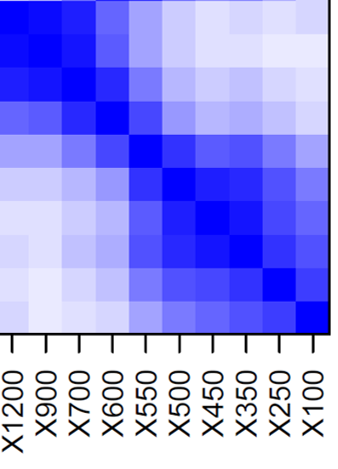
\includegraphics[width=0.35\textwidth]{DRcorr}
}
\subfloat[Imbalanced classes
]{
  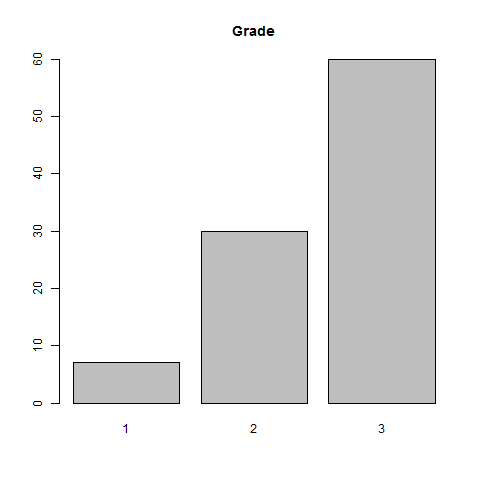
\includegraphics[width=0.45\textwidth]{Gradebarplot}
}
\hspace{0mm}
\subfloat[Empty cells]{
  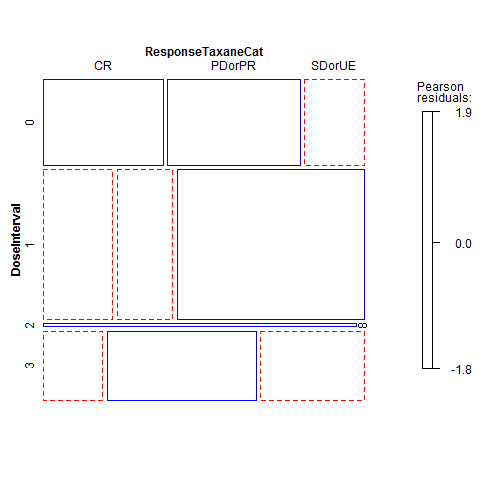
\includegraphics[width=0.45\textwidth]{EmptyCell}
}
\end{figure}


\begin{figure}[h]
\caption{MANOVA Pairwise Contrasts}
\centering
\subfloat[Estimated Contrasts
]{
  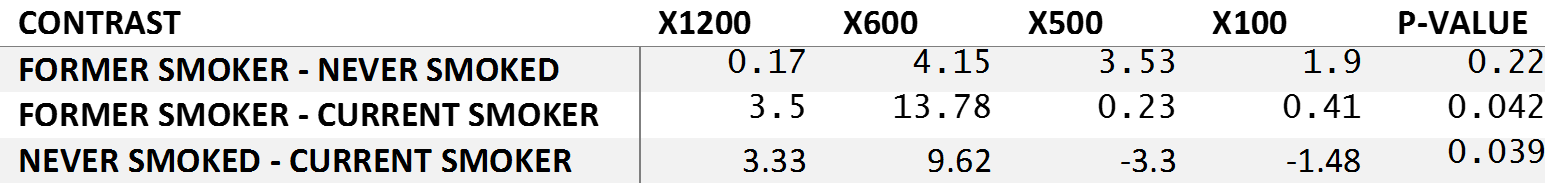
\includegraphics[width=0.95\textwidth]{Contrast}
}
\hspace{0mm}
\subfloat[Boxplots show the distributions of the dose-response variables conditional on smoking status]{
  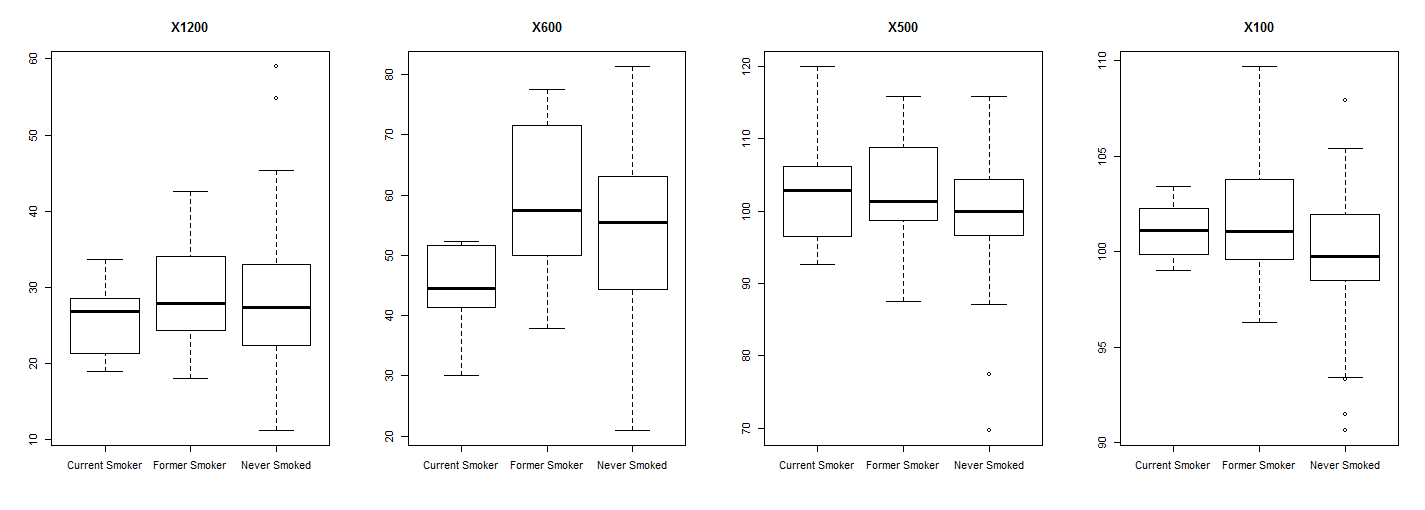
\includegraphics[width=0.95\textwidth]{boxplots}
}
\end{figure}


\begin{figure}[h]
\caption{Two way MANOVA}
\centering
\subfloat[Mosaic plot of Race by Smoking Status]{
  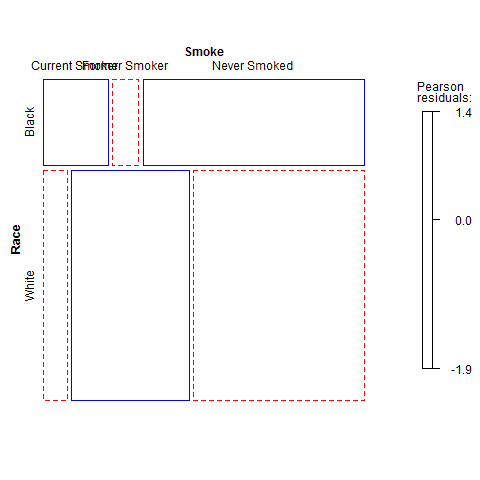
\includegraphics[width=0.45\textwidth]{Race_Smoke}
}
\hspace{10mm}
\subfloat[Two way MANOVA results]{
  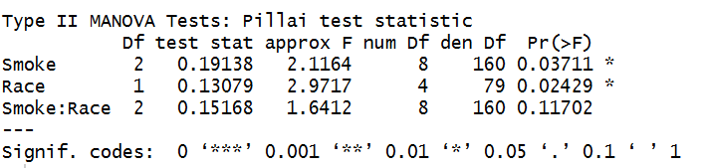
\includegraphics[width=0.45\textwidth]{2wayMANOVA}
}
\end{figure}
\clearpage
}

\begin{table}[ht]
\caption{Multiple MANOVA P-values}
\centering
\begin{tabular}{rlrrr}
  \hline
 & Variable & P-Value & Rank & BHCV \\ 
  \hline
1 & Race & 0.00 &   1 & 0.01 \\ 
  2 & Smoke & 0.01 &   2 & 0.01 \\ 
  3 & Neuropathy & 0.30 &   3 & 0.02 \\ 
  4 & Age & 0.31 &   4 & 0.03 \\ 
  5 & ER & 0.38 &   5 & 0.04 \\ 
  6 & Regimen & 0.40 &   6 & 0.04 \\ 
  7 & TotalWeeks & 0.45 &   7 & 0.05 \\ 
  8 & ERorPR & 0.46 &   8 & 0.06 \\ 
  9 & Menopause & 0.51 &   9 & 0.07 \\ 
  10 & Grade & 0.55 &  10 & 0.07 \\ 
  11 & Myalgia & 0.62 &  11 & 0.08 \\ 
  12 & StagePre & 0.67 &  12 & 0.09 \\ 
  13 & Neutropenia & 0.77 &  13 & 0.10 \\ 
  14 & FollowupStatus & 0.77 &  14 & 0.10 \\ 
  15 & NumCycles & 0.77 &  15 & 0.11 \\ 
  16 & DoseInterval & 0.81 &  16 & 0.12 \\ 
  17 & StageFinal & 0.84 &  17 & 0.13 \\ 
  18 & ResponseNonTaxane & 0.89 &  18 & 0.14 \\ 
  19 & HER2 & 0.97 &  19 & 0.14 \\ 
  20 & ResponseTaxane & 0.97 &  20 & 0.15 \\ 
   \hline
\end{tabular}
\end{table}

\subsection{Clinical data and AC50}

We ran separate simple linear regressions of AC50 on each clinical variable of interest to explore the extent to which AC50 is linearly associated with the in-vivo data. A histogram of the AC50 values can be found in the figures folder, along with summary statistics of the distribution.  We were concerned about normality due to our small sample size.  The distribution is approximately normal, but a more thorough check of the normality of residuals may need to be performed.  Our results indicate that while race and smoking status are the most significant compared to the other variables, neither are statistically significant after correcting for multiple comparisons (Table 2). \\

\begin{table}[ht]
\caption{Multiple SLR P-values}
\centering
\begin{tabular}{rlrrr}
  \hline
 & Variable & P-Value & Rank & BHCV \\ 
  \hline
1 & Race & 0.05 &   1 & 0.01 \\ 
  2 & Smoke & 0.09 &   2 & 0.01 \\ 
  3 & Grade & 0.12 &   3 & 0.02 \\ 
  4 & Regimen & 0.24 &   4 & 0.03 \\ 
  5 & FollowupStatus & 0.32 &   5 & 0.04 \\ 
  6 & ER & 0.38 &   6 & 0.04 \\ 
  7 & ERorPR & 0.51 &   7 & 0.05 \\ 
  8 & Menopause & 0.53 &   8 & 0.06 \\ 
  9 & StageFinal & 0.55 &   9 & 0.07 \\ 
  10 & DoseInterval & 0.56 &  10 & 0.07 \\ 
  11 & Neutropenia & 0.61 &  11 & 0.08 \\ 
  12 & HER2 & 0.69 &  12 & 0.09 \\ 
  13 & ResponseTaxane & 0.76 &  13 & 0.10 \\ 
  14 & StagePre & 0.78 &  14 & 0.10 \\ 
  15 & Age & 0.78 &  15 & 0.11 \\ 
  16 & Neuropathy & 0.79 &  16 & 0.12 \\ 
  17 & NumCycles & 0.79 &  17 & 0.13 \\ 
  18 & ResponseNonTaxane & 0.86 &  18 & 0.14 \\ 
  19 & Myalgia & 0.86 &  19 & 0.14 \\ 
  20 & TotalWeeks & 0.88 &  20 & 0.15 \\ 
   \hline
\end{tabular}
\end{table}

Additionally, we conducted a multiple linear regression of AC50 on the clinical data. Our results do not indicate any significance (Table 3). The variables included in this regression were selected over others based on their intuitive potential contribution. Some variables included in the SLR analysis were removed because of multicollinearity.

\begin{table}[ht]
\caption{Estimates and P-Values from the MLR of AC50 on selected variables}
\centering
\begin{tabular}{rrr}
  \hline
 & Estimates & P-Values \\ 
  \hline
Age & -0.00 & 0.97 \\ 
  Menopause & -2.85 & 0.30 \\ 
  Grade2 & 5.10 & 0.20 \\ 
  Grade3 & 6.04 & 0.12 \\ 
  ERorPR & 0.20 & 0.92 \\ 
  Regimen & 0.16 & 0.95 \\ 
  TotalWeeks & -0.39 & 0.35 \\ 
  Stage2\_Pre & -1.52 & 0.68 \\ 
  Stage3\_Pre & -3.59 & 0.35 \\ 
  Stage4\_Pre & -5.60 & 0.16 \\ 
  Stage5\_Pre & 7.85 & 0.35 \\ 
  Stage6\_Pre & -0.61 & 0.89 \\ 
  RaceBlack & -4.80 & 0.28 \\ 
  RaceWhite & -3.05 & 0.47 \\ 
  Smoker & 0.13 & 0.95 \\ 
  Her2Pos & 0.71 & 0.77 \\ 
   \hline
\end{tabular}
\end{table}

\section{Model Fitting}

We propose a model for recovery status (none, partial, full) using ordinal logistic regression with covariates from the in-vivo data. Ordinal logistic regression is used when the response of interest is categorical with ordered levels, as is the case with our recovery status variable. We examine if adding either AC50 or dose-response curves as a covariate improves model AIC, which would indicate that accounting for the clinical data, LCL data were informative in explaining variation in recovery. AIC is a metric that evaluates a model and is used to compare models. A lower AIC indicates a better fit. Our results displayed in Table 4 show that the model with lowest AIC is the baseline model, where neither AC50 nor dose-response curves were included. Adding AC50 appeared to be more informative than adding dose-response curve data. 

\begin{table}[ht]
\caption{Model Fitting Results}
\centering
\begin{tabular}{cc}
\hline
Model & AIC \\
\hline
Baseline & 173.8224 \\
Add IC-50 & 175.1712 \\
Add DRC  &186.7834 \\
\hline
\end{tabular}
\end{table}

\afterpage{%
\begin{figure}[h]
\caption{Cost complexity pruning of a regression tree model}
\centering
\subfloat[The unpruned tree minimizes the cross validation error]{
  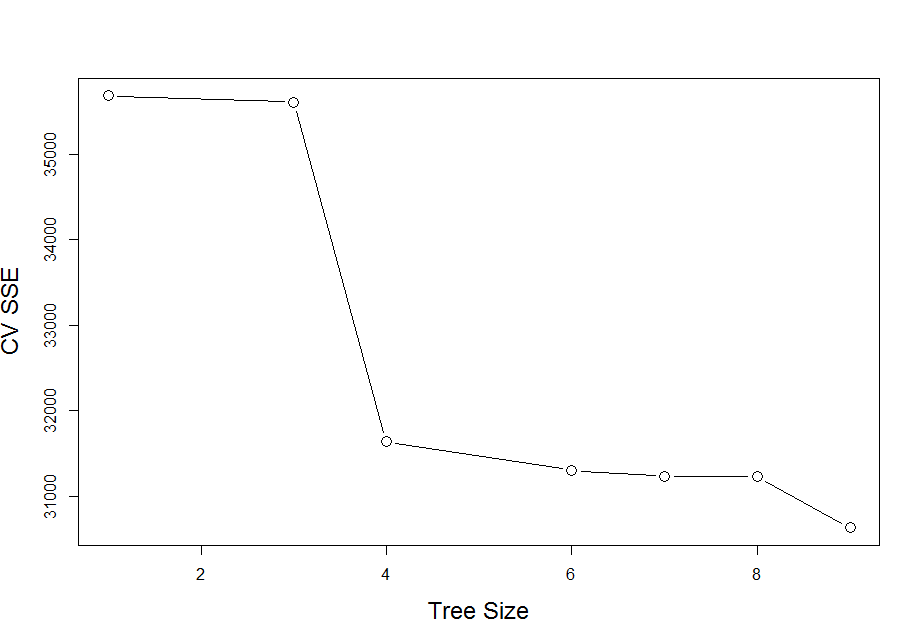
\includegraphics[width=0.45\textwidth]{TreeSizeTune}
}\\[-2ex]
\subfloat[The unpruned regression tree fit to the whole data set]{
  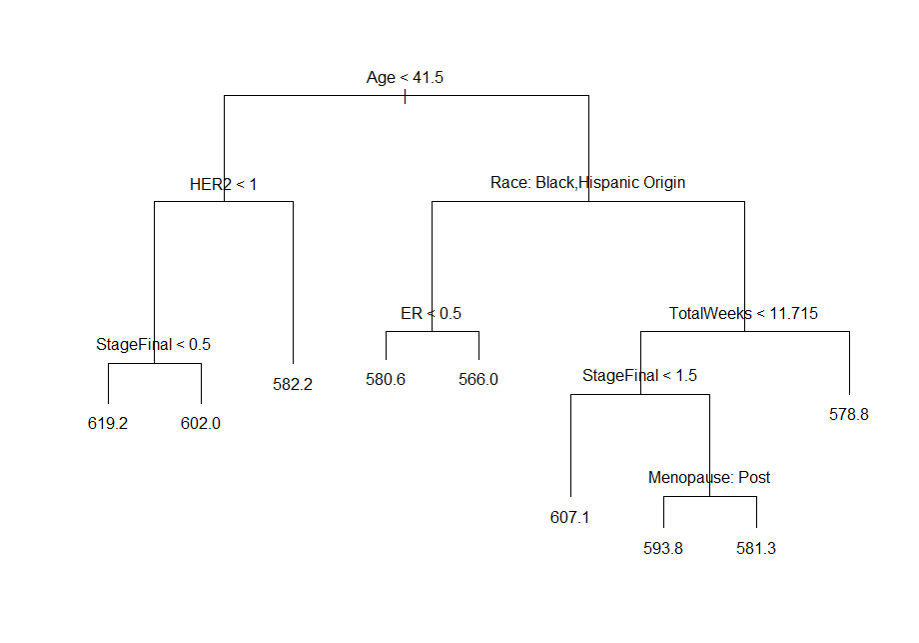
\includegraphics[width=0.85\textwidth]{RegressTree}
}
\end{figure}
\clearpage
}
\afterpage{%
\begin{figure}[h]
\caption{Random Forest Results}
\centering
\subfloat[Tuning of the n and p parameters]{
  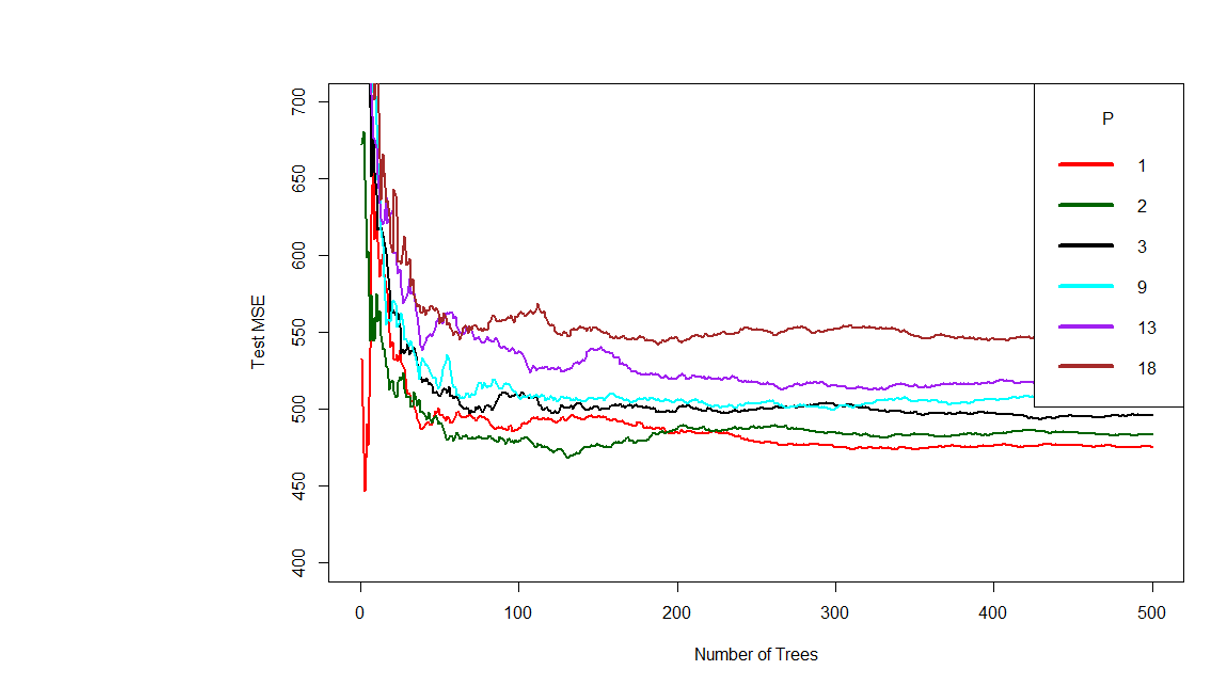
\includegraphics[width=0.55\textwidth]{RFtune}
}
\subfloat[Predicted versus true AC50 values
]{
  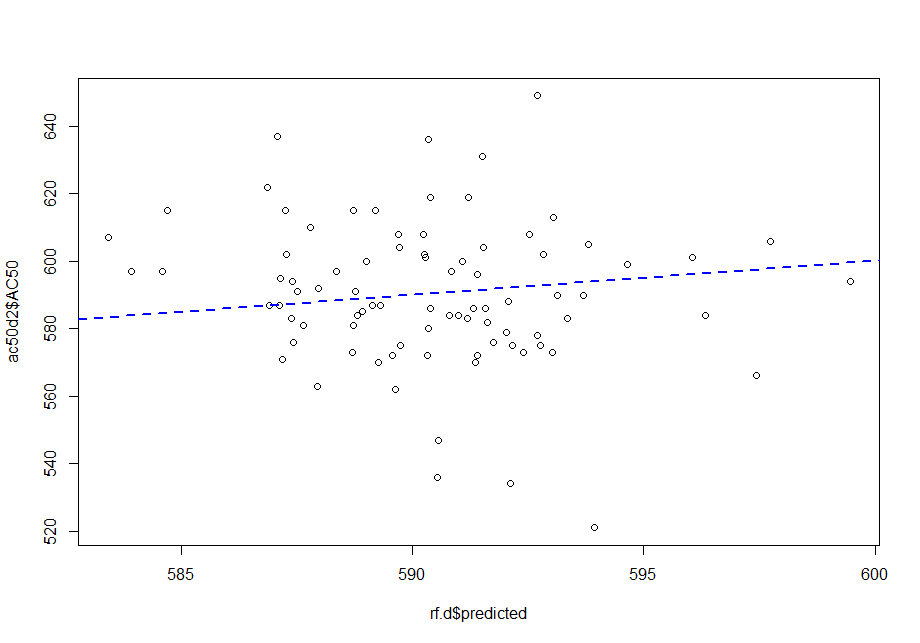
\includegraphics[width=0.45\textwidth]{RFpredVStrue}
}
\hspace{0mm}
\subfloat[Variable importance]{
  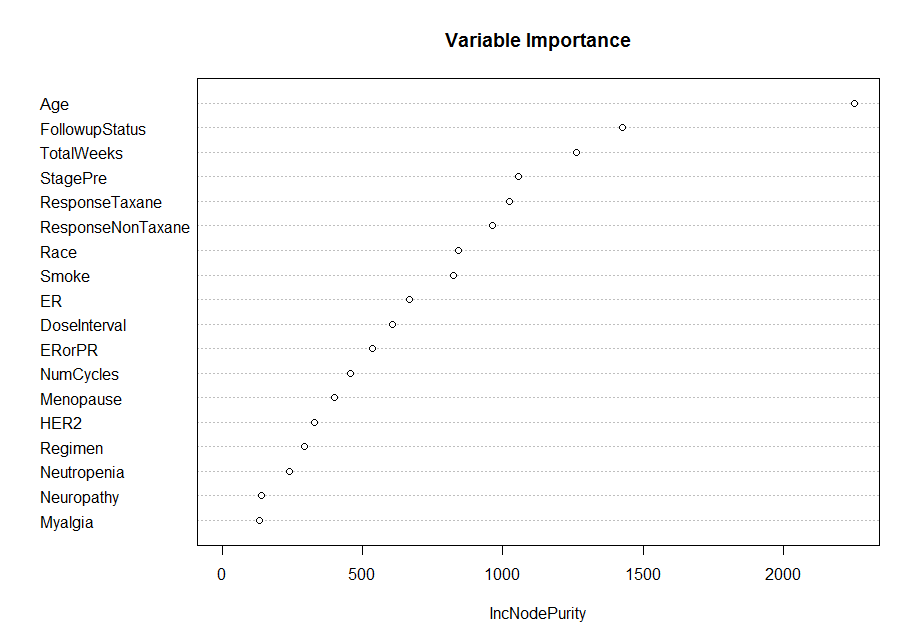
\includegraphics[width=0.85\textwidth]{RFvarImport}
}
\end{figure}
\clearpage
}

\section{Variable Selection}
It was evident from our preliminary analyses that a model that uses the dose-response and patient data as predictors will not have good forward predictive power when predicting in-vivo response to Taxane. Together with Alison we decided to shift our focus from predicting in-vivo response to Taxane to identifying the in-vivo variables in our dataset that are most strongly associated with the dose-response data.  By doing this we hoped to find a few key variables that are associated with the dose-response data after controlling for all other in-vivo data available.  Finding clinical outcome variables that are associated with the dose-response data is of particular interest, due to the fact that no one has analyzed cell line and clinical outcome data from the same patients before, so finding associations between these two data types would suggest that future experiments could elucidate the relationships between these data.  Since a wide variety of LCLs from a range of demographic groups are easily accessed through a variety of archives (1000 Genomes Project, International HapMap Project, etc) and Alison has a collaborator with a group at Duke that can quickly produce more dose-response data, our goal for this project became to identify variables that are strongly associated with the dose-response data and to provide guidance for future experiments for Alison and her collaborators.

We used AC50 values as a summary measure of the dose-response data.  Our objective was to find patient and clinical outcome data that were strongly associated with AC50.  From our multiple linear regression results, it was evident that a linear model was unlikely to identify variables with strong associations.  Instead, because our data exploration suggested tree based methods would perform well, we chose to model using the regression tree and random forests approaches.  Tree based methods were selected over other flexible machine learning models because, unlike most other flexible models, tree based methods provide a measure of which predictors are most important for predicting the response.  Since we were primarily interested in variable selection - as opposed to prediction performance - tree based methods seemed the logical choice.  

\subsection{Regression Tree Model}
A regression tree was fit to the data, using all the in-vivo variables of interest as predictors and AC50 as the response.  Cost complexity pruning was used to select the size of the regression tree to fit to the data.  The regression tree was fit with a grid of alpha values used for cost complexity pruning. This resulted in a range of nested subtrees being fit to the data.  10-fold cross validation was used to select the size of subtree that resulted in the smallest cross validation error.  The tree without any pruning was selected (figure 12a). The cross validated absolute mean error for this model was 55.3, which indicates that the average deviation between the true AC50 values and the predicted AC50 values was 55.3 for held out data. The cross validated $R^2$ for this model was .0001.  Thus, the model has very poor forward prediction performance. To generate a decision tree for interpretation of the relationship between the predictors and AC50, the unpruned regression tree was fit to whole data set (Figure 12b). Age, race, and HER2 status were the most important variables in predicting AC50.  However, clinical outcome variables such as final cancer stage and total weeks of treatment were also important.  Though this method does not have the predictive performance that will be seen in the random forest model, this model results in a highly interpretable tree. For example, young age, HER2 negative patients with a final cancer stage of 0 tend to have high AC50s.  
\subsection{Random Forest Model}
A random forest model with regression trees was fit to the same data.   A grid search was performed for the two parameter values: n, the number of trees used, and p, the number of predictors sampled as split candidates for each split in a tree.  The grid of values for n was the integers from 1 to 1000.  The grid of values for p was (1,2,3,9,13,18). For each pair of parameter values the mean squared error (MSE) was computed for the out of bag (OOB) observations. Figure 13a shows a plot of the OOB MSE for the grid search. A random forest model with these parameters was then fit to the whole data set.  The average decrease in the residual sum of squares that resulted from a split over each variable was calculated.  It appeared as if 300 trees were sufficient to build a model with good forward predictive performance.  Also the models with p=1 consistently performed the best for large values of n.  A model with p=1 and n=1000 was fit to the entire data set.  The average decrease in the OOB residual sum of squares for splits over each variable was calculated.  This is a measure of the importance of each variable for predicting AC50.  Figure 13b shows a plot of the variable importances.  Age is clearly the most important variable, though several clinical outcome variables are important as well.  These include follow up status, total weeks of treatment, stage of cancer before treatment, and interestingly, in-vivo response to Taxane treatment.  For this model, the OOB absolute mean error was 21.9, which indicates that the average deviation between the true AC50 values and the predicted AC50 values was 21.9 for held out data. The OOB $R^2$ was .02.  Thus this model has dramatically better performance than regression trees, but the forward prediction performance is still not good. 


\section{Conclusions}

The primary goal of this study was to uncover any relationships of interest between the clinical outcome and dose-response data. These two types of data have never been available for the same patients and so have never been analyzed before.  This necessitated a thorough exploratory analysis.  Our exploratory analysis suggested that there was substantial complexity in the data, especially due to the fact that much of the patient data was observational and was not generated with standard statistical experimental design.  Because this was the case, careful QC and other data processing was necessary to properly fit our models. Altogether, our exploratory analyses suggested that a flexible machine learning model would fit the relationship between the clinical outcome and dose-response data better than a linear model.  By using MANOVA to look for relationships between the in-vivo data and the dose-response data, we identified two demographic variables - smoking status and race - that showed significant association.  These results may be of use to Alison and her collaborators as they design future experiments looking for differential in-vivo response to Taxane across demographic groups. Diagnostics on our linear models proved very useful for detecting the signal in our dataset.  However, there are more diagnostics that could be done and these may improve our results.  The fact that no variables had significant coefficients in a multiple linear regression relating in-vivo and in-vitro data suggested that a more flexible tree based method might be a better approach.  A regression tree model produced a very interpretable decision tree relating the in-vivo variables to AC50.  Unfortunately, this model has very poor prediction on held out data.  Random forests dramatically improved prediction performance though ultimately no model found a very strong relationship between the in-vivo data and AC50.  However, since random forest did find the strongest relationship between the in-vivo data and AC50 we can use the most important predictor variables in this model to suggest to Alison and collaborators demographic and clinical variables that may be most strongly associated with the in-vitro data. Then, Alison and her collaborators can design experiments more focused on these relationships and perhaps produce more conclusive results.  

The most apparent next step for this analysis would be to build tree based models that uses patient demographic variables and in-vitro variables as predictors and the in-vivo response to Taxane variable as the response.  This would identify in-vitro variables that are potentially strongly associated with the clinical outcome of interest, while controlling for patient demographic variables.

%\newpage
%
%\section*{Appendix A. in-vivo Data Codebook}
%
%\begin{multicols}{2}
%[Include a bar chart, histogram, or box plot, etc. for each individual variable and a short description. ]
%
%\subsection*{Treatment Regimens}
%doseInterval, Regimen (1st or 2nd round of chemo), totalWeeks (total weeks of treatment), NumCycles (?)
%
%\subsection*{Pre-study cancer status}
%Grade (tumor grade), StagePre (Cancer stage before treatment)
%
%\subsection*{Additional patient data}
%Age, Smoking, Race, Menopause, Her2 (Human epidermal growth factor; expression shown to play a role in development and expression of certain aggressive types of breast cancer), ER (Presence of estrogen receptors in cancer cells)
%
%\subsection*{Clinical outcomes}
%Toxicity Reactions (Myalgia, Neropathy, Neutropenia), StagePost (Cancer stage after treatment), percChange, Status, responseTaxane (no recovery, partial recovery, full recovery)
%
%\end{multicols}

\end{document}
































